\documentclass[]{IEEEtran}

% Your packages go here
\usepackage[utf8]{inputenc}
\usepackage{graphicx}
\usepackage{float}
\usepackage{listings}
\usepackage{xcolor}
%listings settings
\definecolor{codegreen}{rgb}{0,0.6,0}
\definecolor{codegray}{rgb}{0.5,0.5,0.5}
\definecolor{codepurple}{rgb}{0.58,0,0.82}
\definecolor{backcolour}{rgb}{0.95,0.95,0.92}
\definecolor{codeblue}{rgb}{0,0.8,0.99}
\definecolor{codeyellow}{rgb}{0.6,0.5,0}


\lstdefinestyle{vim_like}{
  backgroundcolor=\color{backcolour},   
  commentstyle=\color{codegreen},
  keywordstyle=\color{codeyellow},
  numberstyle=\tiny\color{codegray},
  stringstyle=\color{codepurple},
  basicstyle=\ttfamily\footnotesize,
  breakatwhitespace=false,         
  breaklines=true,                 
  captionpos=b,                    
  keepspaces=true,                 
  numbers=left,                    
  numbersep=5pt,                  
  showspaces=false,                
  showstringspaces=false,
  showtabs=false,                  
  tabsize=2
}
\lstset{style=vim_like}

\markboth{MO443 Digital Image Processing}{}

\begin{document}
  \title{Project 1 - Halftoning}
  \author{Thales Mateus Rodrigues Oliveira (RA 148051)
    \thanks{ra148051@students.ic.unicamp.br}
  }
  \maketitle
  
  \begin{abstract}
    In this project, it was given the task of creating a halftoning algorithm to generate images in grayscale and color. To fulfill the requirements, the solution applies error diffusion for neighbor pixels on image sweeping, using approaches listed in the literature. It was able to generate the halftoning images in grayscale and color, and the differences of each error diffusion approach, the pros and cons of the implementation are explained in this report.
  \end{abstract}
  
\section{Introduction}
Halftoning is a technique used for reducing the number of colors used to represent an image, while is desired to keep a good visual perception of its contents for the user. In this work, the implementation of halftoning techniques with error diffusion was realized. For each technique, tests were executed to analyze the quality of the output image, sweeping the image in two different ways. The next sections explains the implemented algorithm, the experiments realized and the output analysis.
\\
The code, along with the input files and the report is delivered in the compressed file THALES\_MATEUS\_RODRIGUES\_OLIVEIRA\_148051.tar, in the Google Classroom.
\section{The Program}
 
The program was implemented with Python 3.7.3. The libraries used and their respective versions are OpenCV 4.1.0 and Numpy 1.16.4.

\subsection{How to execute it}

The project has a Makefile available to help performing some actions on it. The Makefile has 3 basic instructions: clean, build and exec. Clean instruction removes generated images stored in the \textbf{output} folder, the execution code in \textbf{bin} folder and the folders itself. The Build instruction creates the \textbf{output} and \textbf{bin} folders, and moves the source code to \textbf{bin}. The Exec instruction executes the code with images in the \textbf{input} folder. Listing \ref{code:makefile} provides examples of how to execute the three instructions in a terminal.
\begin{lstlisting}[language=sh, caption={Makefile usage example}, label={code:makefile}]
  #clean environment, deletes output and bin folders and their content
  make clean
  
  #prepare the environment for code execution
  make build 

  #executes code
  make exec
\end{lstlisting}

\subsection{Input}

The program does not have an input argument by default, the input images are listed in code, and they are expected to be stored in the \textbf{input} folder. Listing \ref{code:input} shows how images are listed to be executed in code. The $images$ tuple is implemented in $src/main.py$

\begin{lstlisting}[language=Python, caption={Input images inside code}, label={code:input}]
  # for inserting other images, add tem to /input folder and list them here
  images = (
      'baboon',
      'monalisa',
      'peppers',
      'watch'
  )
\end{lstlisting}

\subsection{Output}
The output of the program is a series of halftoning images based on the input ones, changing the error diffusion methods and the sweeping directions. The output images are stored in the \textbf{output} folder, and they are labeled by concatenating the image name, whether is colored or grayscale, the error diffusion method and the sweep order (\textit{e.g.: baboon\_colored\_sierra\_left-to-right.png})

\subsection{Implementation}
The function which implements the halftoning operation is defined in the \textit{src/halftoning.py} file. The file contains a dictionary that lists the approaches used for error diffusion, as mentioned in Figure 1 in the project proposal. Listing \ref{code:masks} shows the implemented dictionary.

\begin{lstlisting}[language=Python, caption={Masks used for error diffusion}, label={code:masks}]
  # Masks used for error propagation
  MASKS = {
      "floyd-steinberg": np.array([
        [0, 0, 7/16],
        [3/16, 5/16, 1/16]]),
      "stevenson-arce": np.array([
        [0, 0, 0, 0, 0, 32/200, 0],
        [12/200, 0, 26/200, 0, 30/200, 0, 16/200],
        [0, 12/200, 0, 26/200, 0, 12/200, 0],
        [5/200, 0, 12/200, 0, 12/200, 0, 5/200]]),
      "burkes": np.array([
        [0, 0, 0, 8/32, 4/32],
        [2/32, 4/32, 8/32, 4/32, 2/32]]),
      "sierra": np.array([
        [0, 0, 0, 5/32, 3/32],
        [2/32, 4/32, 5/32, 4/32, 2/32],
        [0, 2/32, 3/32, 2/32, 0]]),
      "stucki": np.array(
        [[0, 0, 0, 8/42, 4/42],
        [2/42, 4/42, 8/42, 4/42, 2/42],
        [1/42, 2/42, 4/42, 2/42, 1/42]]),
      "jarvis-judice-ninke": np.array([
        [0, 0, 0, 7/48, 5/48],
        [3/48, 5/48, 7/48, 5/48, 3/48],
        [1/48, 3/48, 5/48, 3/48, 1/48]])
  }
\end{lstlisting}
The function \textit{apply\_halftoning} implements the desired operation. It receives the original image, the name of the error diffusion approach, the sweep method (left to right or alternated), and a benchmarking flag to monitor execution time. Listing \ref{code:halftoning} shows keyparts of implementation

\begin{lstlisting}[language=Python, caption={Implementation of halftoning solution}, label={code:halftoning}]
def apply_halftoning(img, err_method="floyd-steinberg", sweep_method=1, benchmarking=False):
  # initialize result array
  result = np.zeros_like(img)
  # separates the masks that could be used
  # (it needs the flip version of mask for alternated sweep)
  m = (0, MASKS[err_method], np.flip(MASKS[err_method], 1))
  # saves mask dimensions to be used when needed
  mask_h, mask_w = m[1].shape
  # saves image dimensions to be used when needed
  img_h, img_w = img.shape
  # it holds the offset of manipulated pixel related to mask
  offset = mask_w//2
  # applies padding to image to make it easier the operations with mask
  img_padded = np.pad(img, ((0, mask_h - 1), (mask_w//2, mask_w//2)), 'constant')

  # default starting direction (left to right)
  direction = 1
  # default index values for sweeping from left to right and right to left
  sweep_options = (0, (0, img_w), (img_w - 1, 0))

  # it sweeps the image from top to bottom
  for j in range(img_h):
      # it sweeps the image from left to right or right to left depending on direction
      beginning, end = sweep_options[direction]
      # do the horizontal sweeping
      for i in range(beginning, end, direction):
          # depending on analyzed pixel, set its result value according to threshold
          if img_padded[j][(i + offset)] < 128:
              result[j][i] = 0
          else:
              result[j][i] = 1

          # calculates associated error
          error = img_padded[j][(i + offset)] - result[j][i]*255
          # propagates error according to mask
          img_padded[j:j+mask_h, i:i+mask_w] = (img_padded[j:j+mask_h, i:i+mask_w]
                                                + (error*m[direction])).astype(np.uint8)
      # it changes from left to right to right to left (vice-versa) depending on the sweep method
      direction *= sweep_method

  # scale the result
  return result*255

\end{lstlisting}
The decisions made in the implementation are explained in the following part.
\subsubsection{Dealing with sweeping directions}
In this solution, it was implemented two approaches: sweeping every line from left to right, and alternating directions when changing from one line to the other. Figure \ref{fig:sweepingmodes} shows the approaches. If the second mentioned method is chosen, the error diffusion mask has to be mirroed in the vertical direction. In order to avoid \textit{if-else} statements when deciding which mask to use for the specific line (the regular or the mirroed one), the tuple \textit{m} holds both masks, and decides which one to use based on the \textit{direction} flag (if \textit{direction} is 1, use the regular mask. If it is -1, use the mirroed one). To sweep the image from right to left, it is also considered the indexes in the loop to decrease. Following the same idea of tuple \textit{m}, the tuple \textit{sweep\_options} is used to set the starting index, the stop index, and the \textit{direction} flag as step.

\begin{figure}[H]
  \centering
  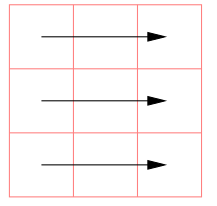
\includegraphics[width=0.4\hsize]{images/sw-left-to-right.png}
  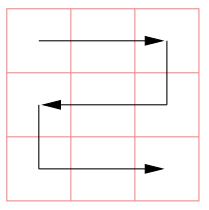
\includegraphics[width=0.4\hsize]{images/sw-alternate.png}
  \caption{Left: Sweeping from left to right. Right: Sweeping alternated}
  \label{fig:sweepingmodes}
\end{figure}

\subsubsection{Image Padding to deal with borders}
In order to deal with pixels in the border of the image, to diffuse the error, the image is padded as the mask propagates the error to its neighbors, as they may not exist for pixels in the border. The padding is done based on the mask properties, such as not diffusing errors to already visited pixels and the dimensions of each mask. The values padded do not matter, as they are not visited.

\subsubsection{Defining the value of the pixel and the error diffusion}
The main ideia of the halftoning algorithm is the following: rather than a simple binarization, in order to create the "feeling" of having more than 2 intensities of a color in the image, an analyzed pixel propagates its information to specific close neighbors. This propagation of information is what we define as error diffusion. Based on a threshold which defines whether a pixel has the maximum or minimum intensity, the resulting pixel value is defined and the error is calculated and passed through specific neighbors with specific weights. That weight is what is defined in the error diffusion masks. The error diffused for the neighbor pixels is proportional to the mentioned weight. After performing these steps to all pixels in the image, the process is done. The steps are the ones inside the two \textit{for} statements in listing \ref{code:halftoning}. They were implemented based on Algorithm 5, presented on the \textit{Enhancement} class of MO443: Introduction to Digital Image Processing course\cite{CLASS:1}.  

\subsubsection{Sweeping the image}
To perform the visit of every pixel, as seen in listing \ref{code:halftoning}, it is used two nested \textit{for} statements. As the author was unable to vectorize the error propagation, the execution time occurs on the second scale. To define the value of the analyzed pixel in the iteration, an  offset is used, as the pixel is in the middle column related to mask.

\section{Experiments}
The \textit{src/main.py} file executes the test pipeline. The idea is the following: for each input image, for each error propagation method, for each sweep order, generate the grayscale and colored halftoning output images. The input images are stored in \textbf{input} folder as mentioned before, and their names and dimensions are listed in table \ref{table:input}. The input images are shown in figure \ref{fig:input-images}

\begin{table}[h!]
\centering
\begin{center}
\begin{tabular}{ |c|c| } 
 \hline
 Image Names & Dimensions (width x height) \\
 \hline
  baboon\_colored.png &  512 x 512\\ 
 \hline
  monalisa\_colored.png & 256 x 256\\
 \hline
  peppers\_colored.png &  512 x 512\\ 
 \hline
  watch\_colored.png & Vertical 1024 x 768\\
 \hline
\end{tabular}
\caption{Input images used in experiments}
\label{table:input}
\end{center}
\end{table}

\begin{figure}[H]
  \centering
  \includegraphics[width=0.4\hsize]{../input/baboon_colored.png}
  \includegraphics[width=0.4\hsize]{../input/monalisa_colored.png}
  \includegraphics[width=0.4\hsize]{../input/peppers_colored.png}
  \includegraphics[width=0.4\hsize]{../input/watch_colored.png}
  \caption{Input images used in experiments. a) Baboon. b) Monalisa c) Peppers d) Watch}
  \label{fig:input-images}
\end{figure}

The error diffusion approaches are taken from the literature\cite{CLASS:1}. The listing \ref{code:masks} indicates their dimensions and weights. Table \ref{table:masks} lists the approaches names and the masks dimensions.

\begin{table}[h!]
  \centering
  \begin{center}
  \begin{tabular}{ |c|c| } 
   \hline
   Error diffusion method & Mask Dimensions (width x height) \\
   \hline
    Floyd and Steinberg &  3 x 2\\ 
   \hline
    Stevenson and Arce & 7 x 4\\
   \hline
    Burkes &  5 x 2\\ 
   \hline
    Sierra & 5 x 3\\
   \hline
    Stucki & 5 x 3\\
   \hline
    Jarvis, Judice and Ninke & 5 x 3 \\ 
   \hline
  \end{tabular}
  \caption{Error diffusion methods used in experiments}
  \label{table:masks}
  \end{center}
  \end{table}

As we have 4 input images, 6 error diffusion methos, 2 sweep modes and it generates 2 output images (grayscale and colored), we have 96 images of output. The output images are stored in the \textbf{output} folder.

\section{Discussion}
This section is organized in four parts. The first part analyses the output images when compared to the original input. The second part takes into consideration the differences of sweeping modes. The third one does the comparisons between the error propagation methods. To sum up, the pros and cons of the implementation.

\subsection{Effectiveness of the technique}
In order to check if the premise of the implementation was achieved, the comparison between input and output images is needed. The figures \ref{fig:effect-baboon}, \ref{fig:effect-monalisa}, \ref{fig:effect-peppers}, \ref{fig:effect-watch} places input and output images together, for all the input images used in the experiments, showing a variety of methods and sweeping orders. 

\begin{figure}[H]
  \centering
  \includegraphics[width=0.4\hsize]{../input/baboon_colored.png}
  \includegraphics[width=0.4\hsize]{../output/baboon_grayscale_floyd-steinberg_left-to-right.png}
  \includegraphics[width=0.4\hsize]{../output/baboon_colored_jarvis-judice-ninke_alternate.png}
  \caption{Baboon images manipulated in experiments. a) Input. b) grayscale by using Floyd and Steinberg, left to right c) colored by using Jarvis, Judice and Ninke, alternate}
  \label{fig:effect-baboon}
\end{figure}

It is interesting to notice, from those images, that the output images are closely related to the input images, even though it is used only the maximum and minimum values of grayscale and color channels. The error diffusion works well in applying the feeling of having multiple intensities of colors, notwithstanding we can still see points or regions with points in the output (\textit{e.g.:} monalisa (grayscale and colored), baboon (grayscale), peppers (colored)).  

\begin{figure}[H]
  \centering
  \includegraphics[width=0.4\hsize]{../input/monalisa_colored.png}
  \includegraphics[width=0.4\hsize]{../output/monalisa_grayscale_stevenson-arce_alternate.png}
  \includegraphics[width=0.4\hsize]{../output/monalisa_colored_sierra_left-to-right.png}
  \caption{Monalisa images manipulated in experiments. a) Input. b) grayscale by using Stevenson and Arce, alternate c) Colored by using Sierra, left to right}
  \label{fig:effect-monalisa}
\end{figure}

\begin{figure}[H]
  \centering
  \includegraphics[width=0.4\hsize]{../input/peppers_colored.png}
  \includegraphics[width=0.4\hsize]{../output/peppers_grayscale_stucki_left-to-right.png}
  \includegraphics[width=0.4\hsize]{../output/peppers_colored_burkes_alternate.png}
  \caption{Peppers images manipulated in experiments. a) Input. b) Grayscale by using Stucki, left to right c) Colored by using Burkes, alternate }
  \label{fig:effect-peppers}
\end{figure}

Furthermore, the output images maintain the contrast seen in the input ones. It is clear that the error diffusion generates outputs which differs a lot of the process of binarization, in which necessary information of image is lost from the quantization according to a specific threshold. 

\begin{figure}[H]
  \centering
  \includegraphics[width=0.4\hsize]{../input/watch_colored.png}
  \includegraphics[width=0.4\hsize]{../output/watch_grayscale_jarvis-judice-ninke_left-to-right.png}
  \includegraphics[width=0.4\hsize]{../output/watch_colored_floyd-steinberg_alternate.png}
  \caption{Watch images manipulated in experiments. a) Input. b) Grayscale by using Jarvis, Judice and Ninke, left to right. c) Colored by using Floyd and Steinberg, alternate. }
  \label{fig:effect-watch}
\end{figure}

\subsection{Sweeping mode differences}

For sweeping mode comparisons, an ideia is to place side by side output images related to the same input and same error diffusion method, and comparing them visually. As the report does not include the images in its real dimensions, it is encouraged to the reader to access the images in the \textbf{output} folder for further inspection. Figures \ref{fig:sweep-baboon}, \ref{fig:sweep-monalisa}, \ref{fig:sweep-peppers} and \ref{fig:sweep-watch} shows 4 output images for every input image, created using the two sweep methods, in grayscale and color.

\begin{figure}[H]
  \centering
  \includegraphics[width=0.4\hsize]{../output/baboon_grayscale_floyd-steinberg_left-to-right.png}
  \includegraphics[width=0.4\hsize]{../output/baboon_grayscale_floyd-steinberg_alternate.png}
  \includegraphics[width=0.4\hsize]{../output/baboon_colored_floyd-steinberg_left-to-right.png}
  \includegraphics[width=0.4\hsize]{../output/baboon_colored_floyd-steinberg_alternate.png}
  \caption{Baboon images manipulated in experiments. a) Grayscale by using Floyd and Steinberg, left to right. b) Grayscale by using Floyd and Steinberg, alternate. c) Colored by using Floyd and Steinberg, left to right. d) Colored by using Floyd and Steinberg, alternate.}
  \label{fig:sweep-baboon}
\end{figure}

The differences are subtle, which makes it difficult to notice in the report, but by inspecting the original ones it is possible to see, for the baboon image input, that the sweep order from left to right creates more visible error points (\textit{e.g.: }yellow and green\textit{-ish} points are bigger in the nose of the baboon) than the alternate sweep. For their grayscale versions, the differences are harder to notice but the same effect is observable (if image is \textit{zoomed-in}).

\begin{figure}[H]
  \centering
  \includegraphics[width=0.4\hsize]{../output/monalisa_grayscale_stucki_left-to-right.png}
  \includegraphics[width=0.4\hsize]{../output/monalisa_grayscale_stucki_alternate.png}
  \includegraphics[width=0.4\hsize]{../output/monalisa_colored_stucki_left-to-right.png}
  \includegraphics[width=0.4\hsize]{../output/monalisa_colored_stucki_alternate.png}
  \caption{Monalisa images manipulated in experiments. a) Grayscale by using Stucki, left to right. b) Grayscale by using Stucki, alternate. c) Colored by using Stucki, left to right. d) Colored by using Stucki, alternate.}
  \label{fig:sweep-monalisa}
\end{figure}

As the monalisa image input is smaller compared to the other ones, it is difficult to spot any differences between the sweep methods.

\begin{figure}[H]
  \centering
  \includegraphics[width=0.4\hsize]{../output/peppers_grayscale_stevenson-arce_left-to-right.png}
  \includegraphics[width=0.4\hsize]{../output/peppers_grayscale_stevenson-arce_alternate.png}
  \includegraphics[width=0.4\hsize]{../output/peppers_colored_stevenson-arce_left-to-right.png}
  \includegraphics[width=0.4\hsize]{../output/peppers_colored_stevenson-arce_alternate.png}
  \caption{Peppers images manipulated in experiments. a) Grayscale by using Stevenson and Arce, left to right. b) Grayscale by using Stevenson and Arce, alternate. c) Colored by using Stevenson and Arce, left to right. d) Colored by using Stevenson and Arce, alternate.}
  \label{fig:sweep-peppers}
\end{figure}

In the peppers case, the differences are more visible in the colored examples. As the background is black, the error diffusion is clearly spotted in the bottom of the image (green blur). For the left to right sweep, the blur are is bigger than in the alternate sweep, and it has the "bottom-to-right" direction, as expected from the mask characteristics and the sweep order. For the alternate sweep, the blur area is more "self-contained", as the propagation happens from left to right and right to left, so the error is diffused to the boundaries of the pepper itself, giving the feeling of more correctude. The error propagation is also clearer in this image for the grayscale cases, as we can see from the white spots in the black background.

\begin{figure}[H]
  \centering
  \includegraphics[width=0.4\hsize]{../output/watch_grayscale_burkes_left-to-right.png}
  \includegraphics[width=0.4\hsize]{../output/watch_grayscale_burkes_alternate.png}
  \includegraphics[width=0.4\hsize]{../output/watch_colored_burkes_left-to-right.png}
  \includegraphics[width=0.4\hsize]{../output/watch_colored_burkes_alternate.png}
  \caption{Watch images manipulated in experiments. a) Grayscale by using Burkes, left to right. b) Grayscale by using Burkes, alternate. c) Colored by using Burkes, left to right. d) Colored by using Burkes, alternate.}
  \label{fig:sweep-watch}
\end{figure}

The same effects noticed in the peppers image appears here for the colored output. Some error is spotted in the "Z arrow" in the image for left to right sweep, while the same error does not appear in the alternate one. Surprisingly, for the grayscale output and Burkes mask, the written text in the left-to-right image has better quality than in the alternate one.

In the majority of cases, the alternate sweep obtained greater quality results, as it tries to compensate the error propagation to both directions.

\subsection{Error Diffusion Methods}
When analyzing the approaches listed in the literature to solve the problem, it is interesting to analyze them side-by-side. To do so, it is chosen colored or grayscale versions of a specific output, and a fixed sweep method, in this case, alternate. Then all solution proposals are grouped. Figures \ref{fig:methods-baboon}, \ref{fig:methods-monalisa}, \ref{fig:methods-peppers} and \ref{fig:methods-watch} shows 6 output images for each input, alternating the error diffusion methods.

\begin{figure}[H]
  \centering
  \includegraphics[width=0.4\hsize]{../output/baboon_colored_floyd-steinberg_alternate.png}
  \includegraphics[width=0.4\hsize]{../output/baboon_colored_stevenson-arce_alternate.png}
  \includegraphics[width=0.4\hsize]{../output/baboon_colored_burkes_alternate.png}
  \includegraphics[width=0.4\hsize]{../output/baboon_colored_sierra_alternate.png}
  \includegraphics[width=0.4\hsize]{../output/baboon_colored_stucki_alternate.png}
  \includegraphics[width=0.4\hsize]{../output/baboon_colored_jarvis-judice-ninke_alternate.png}
  \caption{Baboon images manipulated in experiments. a) Colored by using Floyd and Steiberg, alternate. b) Colored by using Stevenson and Arce, alternate. c) Colored by using Burkes, alternate. d) Colored by using Sierra, alternate. e) Colored by using Stucki, alternate. f) Colored by using Jarvis, Judice and Ninke, alternate. }
  \label{fig:methods-baboon}
\end{figure}

For all error diffusion approaches, the main objective is achieved, but each of them have their peculiarity. With Floyd and Steinberg method, we can see the error more clearly as color points that don't fit to their background (yellow and green points in baboon nose, red points in its blue face). Stevenson and Arce highlights the contours, while we have the similar visibility of errors of Floyd and Steinberg. For Burkes, the error is less noticeable, and the contours of baboon face are atenuated a bit, as the mask is short. For Stucki, Sierra and Jarvis, Judice and Ninke, the visibility of errors is also reduced, and the contours are more visible, as the mask is bigger.   

\begin{figure}[H]
  \centering
  \includegraphics[width=0.4\hsize]{../output/monalisa_grayscale_floyd-steinberg_alternate.png}
  \includegraphics[width=0.4\hsize]{../output/monalisa_grayscale_stevenson-arce_alternate.png}
  \includegraphics[width=0.4\hsize]{../output/monalisa_grayscale_burkes_alternate.png}
  \includegraphics[width=0.4\hsize]{../output/monalisa_grayscale_sierra_alternate.png}
  \includegraphics[width=0.4\hsize]{../output/monalisa_grayscale_stucki_alternate.png}
  \includegraphics[width=0.4\hsize]{../output/monalisa_grayscale_jarvis-judice-ninke_alternate.png}
  \caption{Monalisa images manipulated in experiments. a) Grayscale by using Floyd and Steiberg, alternate. b) Grayscale by using Stevenson and Arce, alternate. c) Grayscale by using Burkes, alternate. d) Grayscale by using Sierra, alternate. e) Grayscale by using Stucki, alternate. f) Grayscale by using Jarvis, Judice and Ninke, alternate. }
  \label{fig:methods-monalisa}
\end{figure}

For Monalisa, as the image is smaller, the differences are more difficult to grasp. But is is observable that the Floyd and Steinberg image has more noise than the other ones, and the Stevenson and Arce gives the feeling of having greater contrast. 

The pepper output images have the same characteristics of the baboon image, already listed.

For the watch images, all of them reproduces the image well, being able to distinguish their details, even though the noise feeling is greater in the Floyd and Steinberg approach. All of them fail to reproduce the black background correctly. 

\begin{figure}[H]
  \centering
  \includegraphics[width=0.4\hsize]{../output/peppers_colored_floyd-steinberg_alternate.png}
  \includegraphics[width=0.4\hsize]{../output/peppers_colored_stevenson-arce_alternate.png}
  \includegraphics[width=0.4\hsize]{../output/peppers_colored_burkes_alternate.png}
  \includegraphics[width=0.4\hsize]{../output/peppers_colored_sierra_alternate.png}
  \includegraphics[width=0.4\hsize]{../output/peppers_colored_stucki_alternate.png}
  \includegraphics[width=0.4\hsize]{../output/peppers_colored_jarvis-judice-ninke_alternate.png}
  \caption{Peppers images manipulated in experiments. a) Colored by using Floyd and Steiberg, alternate. b) Colored by using Stevenson and Arce, alternate. c) Colored by using Burkes, alternate. d) Colored by using Sierra, alternate. e) Colored by using Stucki, alternate. f) Colored by using Jarvis, Judice and Ninke, alternate. }
  \label{fig:methods-peppers}
\end{figure}

 

\begin{figure}[H]
  \centering
  \includegraphics[width=0.4\hsize]{../output/watch_grayscale_floyd-steinberg_alternate.png}
  \includegraphics[width=0.4\hsize]{../output/watch_grayscale_stevenson-arce_alternate.png}
  \includegraphics[width=0.4\hsize]{../output/watch_grayscale_burkes_alternate.png}
  \includegraphics[width=0.4\hsize]{../output/watch_grayscale_sierra_alternate.png}
  \includegraphics[width=0.4\hsize]{../output/watch_grayscale_stucki_alternate.png}
  \includegraphics[width=0.4\hsize]{../output/watch_grayscale_jarvis-judice-ninke_alternate.png}
  \caption{Watch images manipulated in experiments. a) Grayscale by using Floyd and Steiberg, alternate. b) Grayscale by using Stevenson and Arce, alternate. c) Grayscale by using Burkes, alternate. d) Grayscale by using Sierra, alternate. e) Grayscale by using Stucki, alternate. f) Grayscale by using Jarvis, Judice and Ninke, alternate.}
  \label{fig:methods-watch}
\end{figure}

\subsection{Pros and Cons}
All methods achieve the objective of representing the original image characteristics with only two intensities per channel, each one having its own peculiarity. Floyd and Steinberg images have the least visible quality, as the propagated error is visible in the output, giving the feeling of being \textit{noisy}. Stevenson and Arce images are very interesting, as they highlights the contours of objects in the image. The other methods proposed generate images with great quality, not interfering a lot in its original contours. In general, the technique performs bad when propagating error to uniform spaces, as the blackbackgrounds in our experiments.

Enabling the benchmarking flag, it was able to check the execution time for every output image. For each image channel, the execution time varied from 0.7 seconds for the monalisa image (smallest dimensions) to 9 seconds for the watch image (biggest dimensions), executing in a Intel(R) Core(TM) i7-4720HQ CPU @ 2.60GHz processor. As the technique sweeps through every pixel to do the error diffusion, the execution time is penalyzed.


\section{Conclusion}
The application of halftoning techniques to generate output images with similar characteristics of their inputs with only two levels of color intensity per channel was possible thanks to error propagation through image sweeping.

The usage of different input images, error diffusion techniques and sweep modes made it possible to analyze each approach's strength.

\bibliography{ref-project} 
\bibliographystyle{ieeetr}

\end{document}
